\documentclass[aspectratio=169,10pt]{beamer}

% -----------------------------------------------------------------------------
% LifeLink: Intelligent Blood Donation & Emergency Matching Platform
% LaTeX Beamer Presentation for Overleaf / Academic Project Defense
% -----------------------------------------------------------------------------

% Theme & Styling
\usetheme{Madrid}
\usecolortheme{whale}

% Typography & Packages
\usepackage[utf8]{inputenc}
\usepackage[T1]{fontenc}
\usepackage{lmodern}
\usepackage{amsmath,amssymb}
\usepackage{booktabs}
\usepackage{listings}
\usepackage{tikz}
\usetikzlibrary{shapes.geometric, arrows, positioning, fit, backgrounds, calc}
\usepackage{hyperref}
\usepackage{graphicx}
\usepackage{microtype}
\usepackage{colortbl}

% Image directory configuration for Overleaf
% If you upload images to Overleaf, place them in the root or in an 'images/' folder:
\graphicspath{{images/}{./}}

% Color Palette Definition
\definecolor{MedicalRed}{RGB}{220, 38, 38}
\definecolor{DarkSlate}{RGB}{15, 23, 42}
\definecolor{SoftSlate}{RGB}{51, 65, 85}
\definecolor{LightBg}{RGB}{248, 250, 252}
\definecolor{AccentBlue}{RGB}{37, 99, 235}
\definecolor{SuccessGreen}{RGB}{22, 163, 74}
\definecolor{CodeBg}{RGB}{241, 245, 249}

% Beamer Color Customizations
\setbeamercolor{palette primary}{bg=DarkSlate, fg=white}
\setbeamercolor{palette secondary}{bg=SoftSlate, fg=white}
\setbeamercolor{palette tertiary}{bg=MedicalRed, fg=white}
\setbeamercolor{structure}{fg=MedicalRed}
\setbeamercolor{frametitle}{bg=DarkSlate, fg=white}
\setbeamercolor{title}{bg=DarkSlate, fg=white}
\setbeamercolor{block title}{bg=MedicalRed, fg=white}
\setbeamercolor{block body}{bg=CodeBg, fg=DarkSlate}
\setbeamercolor{block title alerted}{bg=AccentBlue, fg=white}
\setbeamercolor{block body alerted}{bg=CodeBg, fg=DarkSlate}
\setbeamercolor{block title example}{bg=SuccessGreen, fg=white}
\setbeamercolor{block body example}{bg=CodeBg, fg=DarkSlate}

% JavaScript Definition for listings
\lstdefinelanguage{JavaScript}{
  keywords={typeof, new, true, false, catch, function, return, null, catch, switch, var, if, in, while, do, else, case, break, const, let, async, await, export},
  keywordstyle=\color{AccentBlue}\bfseries,
  ndkeywords={class, export, boolean, throw, implements, import, this},
  ndkeywordstyle=\color{DarkSlate}\bfseries,
  identifierstyle=\color{DarkSlate},
  sensitive=false,
  comment=[l]{//},
  morecomment=[s]{/*}{*/},
  commentstyle=\color{SoftSlate}\itshape,
  stringstyle=\color{MedicalRed}\ttfamily,
  morestring=[b]',
  morestring=[b]"
}

% Code Listing Configuration
\lstset{
    language=JavaScript,
    backgroundcolor=\color{CodeBg},
    basicstyle=\ttfamily\scriptsize\color{DarkSlate},
    keywordstyle=\color{AccentBlue}\bfseries,
    stringstyle=\color{MedicalRed},
    commentstyle=\color{SoftSlate}\itshape,
    breaklines=true,
    showstringspaces=false,
    frame=single,
    rulecolor=\color{SoftSlate!30},
    numbers=none
}

% Metadata
\title[\textbf{LifeLink Platform}]{\textbf{LifeLink: Intelligent Blood Donation \& Emergency Matching Platform}}
\subtitle{A Full-Stack Healthcare Database Management System (DBMS)}
\author[Project Presentation]{\textbf{Department of Computer Science \& Engineering}}
\institute[LifeLink Health Stack]{Database Management Systems (DBMS) Laboratory \\ Full-Stack HealthTech Infrastructure}
\date[\today]{Final Project Review \& Technical Presentation}

% =============================================================================
\begin{document}

% Slide 1: Title Slide
\begin{frame}
    \titlepage
\end{frame}

% Slide 2: Table of Contents
\begin{frame}{Agenda \& Presentation Roadmap}
    \tableofcontents
\end{frame}

% =============================================================================
\section{Executive Overview \& Motivation}
% =============================================================================

\begin{frame}{1. Problem Statement \& Healthcare Motivation}
    \begin{columns}[T]
        \begin{column}{0.5\textwidth}
            \begin{block}{\textbf{The Critical Healthcare Challenge}}
                \begin{itemize}
                    \item \textbf{Emergency Time Delay}: Critical trauma victims often face delays of 30--90 minutes in securing matching blood.
                    \item \textbf{Opaque Hospital Inventory}: Lack of real-time visibility into blood bank stock across regional medical centers.
                    \item \textbf{Supply-Demand Imbalance}: Severe shortages of rare blood types ($O-$, $AB-$) combined with seasonal wastage.
                    \item \textbf{Disjoint Communication}: No automated bridge between hospitals and volunteer donors.
                \end{itemize}
            \end{block}
        \end{column}
        \begin{column}{0.5\textwidth}
            \begin{alertblock}{\textbf{The LifeLink Solution}}
                \begin{itemize}
                    \item \textbf{Zero-Latency Triage}: Instant broadcast of emergency blood requirements with automated compatibility matching.
                    \item \textbf{Live 8-Group Matrix}: Real-time tracking of hospital stocks ($A+, A-, B+, B-, AB+, AB-, O+, O-$).
                    \item \textbf{Geospatial Matching Engine}: Mathematical Haversine proximity computation connecting nearby donors.
                    \item \textbf{Enterprise DBMS Integrity}: 100\% BCNF normalization, ACID guarantees, and automated cascade lifecycles.
                \end{itemize}
            \end{alertblock}
        \end{column}
    \end{columns}
\end{frame}

% =============================================================================
\section{System Architecture \& Process Pipeline}
% =============================================================================

\begin{frame}{2. System Architecture (3-Tier Enterprise Design)}
    \begin{center}
    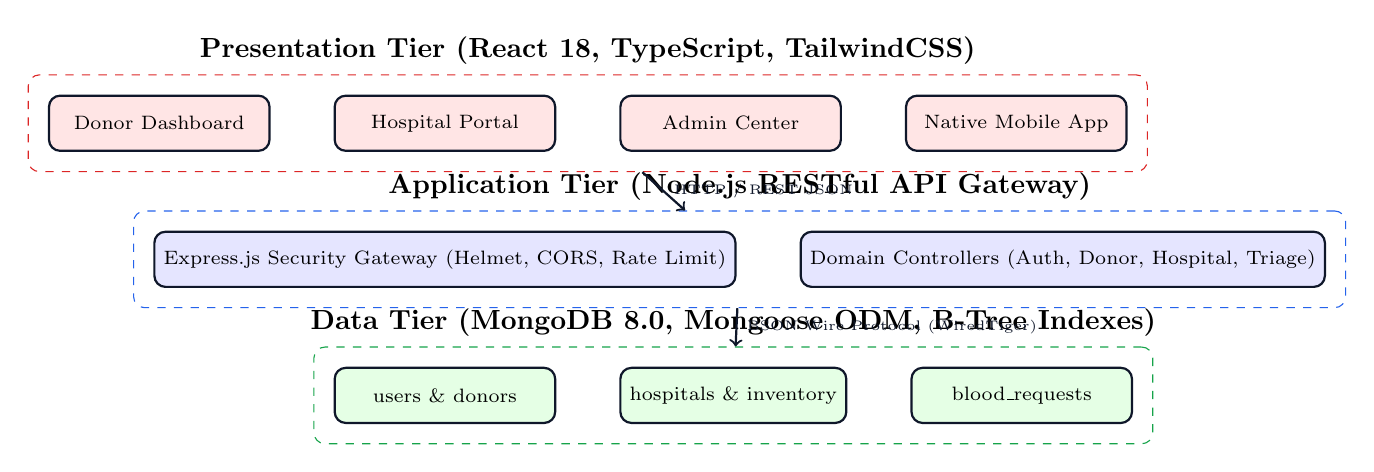
\begin{tikzpicture}[
        node distance=0.7cm and 0.8cm,
        box/.style={rectangle, rounded corners, draw=DarkSlate, fill=white, thick, minimum width=2.8cm, minimum height=0.7cm, align=center, font=\scriptsize},
        layer/.style={rectangle, rounded corners, draw=MedicalRed, dashed, inner sep=0.25cm, font=\bfseries\scriptsize}
    ]
        % Presentation Tier
        \node[box, fill=red!10] (client1) {Donor Dashboard};
        \node[box, fill=red!10, right=of client1] (client2) {Hospital Portal};
        \node[box, fill=red!10, right=of client2] (client3) {Admin Center};
        \node[box, fill=red!10, right=of client3] (client4) {Native Mobile App};
        \begin{scope}[on background layer]
            \node[layer, fit=(client1)(client4), label=above:{\textbf{Presentation Tier (React 18, TypeScript, TailwindCSS)}}] (presLayer) {};
        \end{scope}

        % API Gateway Tier
        \node[box, fill=blue!10, below=1.0cm of client2] (gateway) {Express.js Security Gateway (Helmet, CORS, Rate Limit)};
        \node[box, fill=blue!10, right=of gateway] (ctrl) {Domain Controllers (Auth, Donor, Hospital, Triage)};
        \begin{scope}[on background layer]
            \node[layer, draw=AccentBlue, fit=(gateway)(ctrl), label=above:{\textbf{Application Tier (Node.js RESTful API Gateway)}}] (appLayer) {};
        \end{scope}

        % Data Tier
        \node[box, fill=green!10, below=1.0cm of gateway] (db1) {users \& donors};
        \node[box, fill=green!10, right=of db1] (db2) {hospitals \& inventory};
        \node[box, fill=green!10, right=of db2] (db3) {blood\_requests};
        \begin{scope}[on background layer]
            \node[layer, draw=SuccessGreen, fit=(db1)(db3), label=above:{\textbf{Data Tier (MongoDB 8.0, Mongoose ODM, B-Tree Indexes)}}] (dataLayer) {};
        \end{scope}

        % Connections
        \draw[->, thick, DarkSlate] (presLayer) -- (appLayer) node[midway, right, font=\tiny] {HTTP / REST JSON};
        \draw[->, thick, DarkSlate] (appLayer) -- (dataLayer) node[midway, right, font=\tiny] {BSON Wire Protocol (WiredTiger)};
    \end{tikzpicture}
    \end{center}
    \vspace{-0.2cm}
    \begin{exampleblock}{\textbf{Key Engineering Highlight}}
        \scriptsize Strict separation of concerns between presentation, business validation, and atomic database persistence guarantees sub-millisecond transaction execution.
    \end{exampleblock}
\end{frame}

\begin{frame}{3. End-to-End Emergency Matching Flowchart}
    \begin{center}
    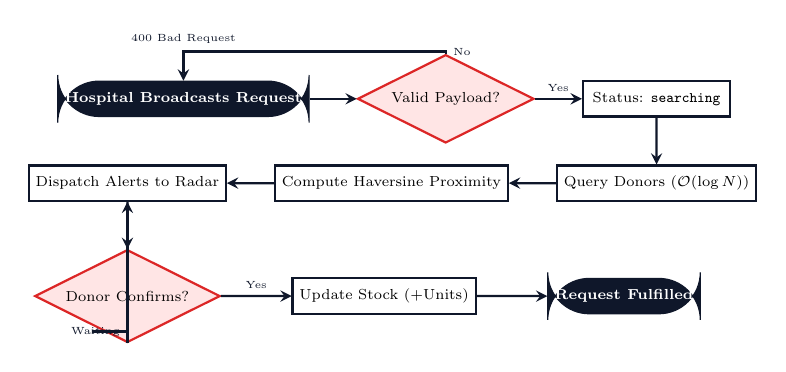
\begin{tikzpicture}[
        scale=0.75, every node/.style={transform shape},
        startstop/.style={rectangle, rounded corners=15pt, minimum width=2.5cm, minimum height=0.6cm, text centered, draw=DarkSlate, fill=DarkSlate, text=white, font=\bfseries\scriptsize},
        process/.style={rectangle, minimum width=2.5cm, minimum height=0.6cm, text centered, draw=DarkSlate, fill=white, thick, font=\scriptsize},
        decision/.style={diamond, aspect=2, text centered, draw=MedicalRed, fill=red!10, thick, font=\scriptsize},
        arrow/.style={thick, ->, >=stealth, DarkSlate}
    ]
        \node (start) [startstop] {Hospital Broadcasts Request};
        \node (val) [decision, right=0.8cm of start] {Valid Payload?};
        \node (save) [process, right=0.8cm of val] {Status: \texttt{searching}};
        \node (query) [process, below=0.8cm of save] {Query Donors ($\mathcal{O}(\log N)$)};
        \node (calc) [process, left=0.8cm of query] {Compute Haversine Proximity};
        \node (alert) [process, left=0.8cm of calc] {Dispatch Alerts to Radar};
        \node (coord) [decision, below=0.8cm of alert] {Donor Confirms?};
        \node (stock) [process, right=1.2cm of coord] {Update Stock (+Units)};
        \node (end) [startstop, right=1.2cm of stock] {Request Fulfilled};

        \draw [arrow] (start) -- (val);
        \draw [arrow] (val) -- node[above, font=\tiny] {Yes} (save);
        \draw [arrow] (val) |- node[right, font=\tiny] {No} ++(0, 0.8) -| node[above, font=\tiny] {400 Bad Request} (start);
        \draw [arrow] (save) -- (query);
        \draw [arrow] (query) -- (calc);
        \draw [arrow] (calc) -- (alert);
        \draw [arrow] (alert) -- (coord);
        \draw [arrow] (coord) -- node[above, font=\tiny] {Yes} (stock);
        \draw [arrow] (coord) |- node[left, font=\tiny] {Waiting} ++(-0.6, -0.6) -| (alert);
        \draw [arrow] (stock) -- (end);
    \end{tikzpicture}
    \end{center}
\end{frame}

% =============================================================================
\section{Database Design \& DBMS Foundations}
% =============================================================================

\begin{frame}{4. Entity-Relationship (ER) Modeling \& Relational Schema}
    \begin{columns}[T]
        \begin{column}{0.5\textwidth}
            \begin{block}{\textbf{Core Database Relations}}
                \scriptsize
                \begin{itemize}
                    \item \textbf{USER}(\underline{user\_id}, name, email, password\_hash, role, created\_at)
                    \item \textbf{DONOR}(\underline{donor\_id}, \underline{user\_id}, blood\_group, phone, latitude, longitude, availability)
                    \item \textbf{HOSPITAL}(\underline{hospital\_id}, \underline{user\_id}, hospital\_name, phone, emergency\_contact, address, latitude, longitude)
                    \item \textbf{BLOOD\_INVENTORY}(\underline{inventory\_id}, \underline{hospital\_id}, blood\_group, units, updated\_at)
                    \item \textbf{BLOOD\_REQUEST}(\underline{request\_id}, \underline{hospital\_id}, blood\_group, units\_required, urgency, status)
                    \item \textbf{NOTIFICATION}(\underline{notification\_id}, recipient\_id, recipient\_role, title, message, is\_read)
                \end{itemize}
            \end{block}
        \end{column}
        \begin{column}{0.5\textwidth}
            \begin{alertblock}{\textbf{Disjoint Subtype Inheritance}}
                \scriptsize
                \textbf{Supertype}: \texttt{USER} contains shared authentication credentials. \\
                \textbf{Subtypes}: \texttt{DONOR} and \texttt{HOSPITAL} specialize based on discriminator \texttt{role}:
                \[ \forall u \in \text{USER},\; \text{role}(u) = \text{'donor'} \iff \exists!\, d \in \text{DONOR} \]
                \[ \forall u \in \text{USER},\; \text{role}(u) = \text{'hospital'} \iff \exists!\, h \in \text{HOSPITAL} \]
            \end{alertblock}
            \begin{exampleblock}{\textbf{Key Constraints}}
                \scriptsize
                \begin{itemize}
                    \item \textbf{Compound Unique Index}: \texttt{\{ hospital\_id: 1, blood\_group: 1 \}} enforces strictly one stock row per blood type.
                    \item \textbf{Domain Integrity}: Enumerated checks for ABO/Rh groups and triage tiers.
                \end{itemize}
            \end{exampleblock}
        \end{column}
    \end{columns}
\end{frame}

\begin{frame}{5. Database Normalization Proofs \& Integrity Constraints}
    \begin{table}[H]
        \centering
        \scriptsize
        \begin{tabular}{lp{4.2cm}p{5.5cm}}
            \toprule
            \textbf{Normal Form} & \textbf{Formal DBMS Rule} & \textbf{LifeLink Implementation Proof} \\
            \midrule
            \textbf{1NF} & Atomic scalar values; no repeating groups. & Blood types stored as distinct tuples in \texttt{blood\_inventory} rather than unindexed array. \\
            \textbf{2NF} & Full functional dependency on candidate key ($PK \to \text{Attributes}$). & No partial key dependencies; all attributes depend on complete single/compound keys. \\
            \textbf{3NF} & Transitive dependency elimination ($X \to Y \land Y \to Z$). & Hospital location/hotline isolated solely in \texttt{HOSPITAL}; not redundantly duplicated in \texttt{BLOOD\_REQUEST}. \\
            \textbf{BCNF} & For every functional dependency $X \to Y$, $X$ must be a superkey. & All determinant attributes across all 6 collections are verified superkeys. \\
            \bottomrule
        \end{tabular}
    \end{table}

    \begin{block}{\textbf{Controlled De-normalization for Emergency Optimization}}
        \scriptsize Index-covered \texttt{\$lookup} aggregation performs single-trip relational joins in $\mathcal{O}(1)$ time, eliminating network overhead during critical trauma triage.
    \end{block}
\end{frame}

\begin{frame}[fragile]{6. ACID Guarantees \& Concurrency Control}
    \begin{columns}[T]
        \begin{column}{0.5\textwidth}
            \begin{block}{\textbf{ACID Transaction Guarantees}}
                \begin{itemize}
                    \item \textbf{Atomicity ($A$)}: Single-document atomic mutations via \texttt{\$set} and \texttt{\$inc}.
                    \item \textbf{Consistency ($C$)}: Schema pre-save hooks and unique B-Tree indexes prevent corrupt states.
                    \item \textbf{Isolation ($I$)}: Read-committed isolation eliminates dirty reads under high concurrent requests.
                    \item \textbf{Durability ($D$)}: WiredTiger Write-Ahead Logging (WAL) guarantees durability.
                \end{itemize}
            \end{block}
        \end{column}
        \begin{column}{0.5\textwidth}
            \begin{alertblock}{\textbf{Race Condition Mitigation (CAS)}}
                \scriptsize
                To prevent negative stock during concurrent emergency allocations, atomic compare-and-swap is applied:
\begin{lstlisting}
// Atomic allocation with safety precondition
await BloodInventory.updateOne(
  { 
    hospital_id: hospId, 
    blood_group: 'O-', 
    units: { $gte: requiredUnits } 
  },
  { $inc: { units: -requiredUnits } }
);
\end{lstlisting}
            \end{alertblock}
        \end{column}
    \end{columns}
\end{frame}

% =============================================================================
\section{Query Optimization \& Relational Algebra}
% =============================================================================

\begin{frame}{7. Core Query Catalog: Relational Algebra vs SQL vs NoSQL}
    \begin{table}[H]
        \centering
        \tiny
        \begin{tabular}{p{2.6cm}p{3.8cm}p{4.2cm}p{1.8cm}}
            \toprule
            \textbf{System Operation} & \textbf{Relational Algebra} & \textbf{Standard ANSI SQL} & \textbf{Index \& Time} \\
            \midrule
            \textbf{User Authentication} & $\sigma[\text{email} = e](\text{USER})$ & \texttt{SELECT * FROM users WHERE email = ? LIMIT 1} & \texttt{IXSCAN} $\mathcal{O}(\log N)$ \\[4pt]
            \textbf{Active Donor Discovery} & $\pi[\text{id, phone, lat, lng}](\sigma[\text{group}=g \land \text{avail}=\text{true}](\text{DONOR}))$ & \texttt{SELECT id, phone, latitude, longitude FROM donors WHERE blood\_group = ? AND availability = true} & \texttt{IXSCAN} (Compound) $\mathcal{O}(\log N)$ \\[4pt]
            \textbf{Emergency Triage Join} & $\pi[\dots](\sigma[\text{group}=g \land \text{status}=\text{'searching'}](\text{REQUEST}) \bowtie \text{HOSPITAL})$ & \texttt{SELECT * FROM blood\_requests r INNER JOIN hospitals h ON r.hospital\_id = h.id WHERE r.blood\_group = ?} & \texttt{IXSCAN} + PK Join $\mathcal{O}(\log N)$ \\[4pt]
            \textbf{Stock Matrix Upsert} & $\text{UPSERT}(\text{INVENTORY}, h \land g, \text{units} \leftarrow u)$ & \texttt{INSERT INTO blood\_inventory \dots ON CONFLICT (hospital\_id, blood\_group) DO UPDATE} & Unique B-Tree Seek $\mathcal{O}(1)$ \\[4pt]
            \textbf{Platform Total Reserve} & $\gamma[\text{blood\_group}, \text{SUM}(\text{units})](\text{INVENTORY})$ & \texttt{SELECT blood\_group, SUM(units) FROM blood\_inventory GROUP BY blood\_group} & Hash Aggregate $\mathcal{O}(N)$ \\
            \bottomrule
        \end{tabular}
    \end{table}
\end{frame}

\begin{frame}[fragile]{8. Topological Referential Cascade Deletion}
    \begin{columns}[T]
        \begin{column}{0.48\textwidth}
            \begin{block}{\textbf{Topological Dependency Ordering}}
                \scriptsize
                Deleting a root \texttt{USER} executes a structured cascade purge across dependent child entities:
                \begin{center}
                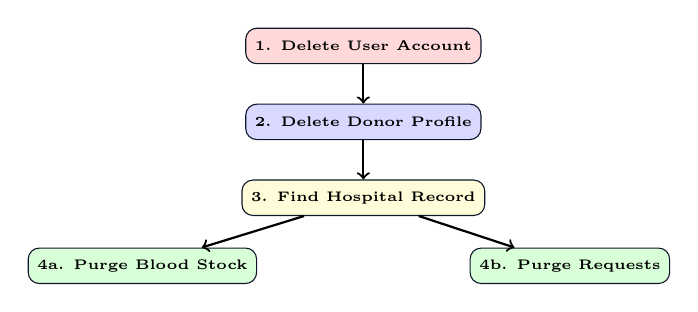
\begin{tikzpicture}[
                    node distance=0.5cm,
                    box/.style={rectangle, rounded corners, draw=DarkSlate, fill=white, font=\tiny\bfseries, minimum height=0.45cm}
                ]
                    \node[box, fill=red!15] (user) {1. Delete User Account};
                    \node[box, fill=blue!15, below=of user] (donor) {2. Delete Donor Profile};
                    \node[box, fill=yellow!15, below=of donor] (hosp) {3. Find Hospital Record};
                    \node[box, fill=green!15, below left=0.4cm and -0.2cm of hosp] (stock) {4a. Purge Blood Stock};
                    \node[box, fill=green!15, below right=0.4cm and -0.2cm of hosp] (req) {4b. Purge Requests};

                    \draw[->, thick] (user) -- (donor);
                    \draw[->, thick] (donor) -- (hosp);
                    \draw[->, thick] (hosp) -- (stock);
                    \draw[->, thick] (hosp) -- (req);
                \end{tikzpicture}
                \end{center}
            \end{block}
        \end{column}
        \begin{column}{0.52\textwidth}
            \begin{alertblock}{\textbf{Cascade Implementation Code}}
\begin{lstlisting}
export const deleteUser = async (req, res, next) => {
  const { user_id } = req.params;
  // 1. Purge linked donor
  await Donor.deleteMany({ user_id });
  // 2. Cascade hospital records
  const hosp = await Hospital.findOne({ user_id });
  if (hosp) {
    await BloodInventory.deleteMany({ 
      hospital_id: hosp._id 
    });
    await BloodRequest.deleteMany({ 
      hospital_id: hosp._id 
    });
    await Hospital.findByIdAndDelete(hosp._id);
  }
  // 3. Purge root user record
  await User.findByIdAndDelete(user_id);
};
\end{lstlisting}
            \end{alertblock}
        \end{column}
    \end{columns}
\end{frame}

% =============================================================================
\section{Geospatial Engine \& Biological Compatibility}
% =============================================================================

\begin{frame}{9. Geospatial Routing: Haversine Trigonometric Model}
    \begin{columns}[T]
        \begin{column}{0.5\textwidth}
            \begin{block}{\textbf{Spherical Trigonometry Formula}}
                \scriptsize
                \[ d = 2R \cdot \text{atan2}\left(\sqrt{a}, \sqrt{1-a}\right) \]
                \[ a = \sin^2\left(\frac{\Delta \phi}{2}\right) + \cos(\phi_1)\cos(\phi_2)\sin^2\left(\frac{\Delta \lambda}{2}\right) \]
                \begin{itemize}
                    \item $\phi_1, \phi_2$: Latitude coordinates in radians.
                    \item $\lambda_1, \lambda_2$: Longitude coordinates in radians.
                    \item $R$: Earth mean radius ($6,371\text{ km}$).
                \end{itemize}
            \end{block}
        \end{column}
        \begin{column}{0.5\textwidth}
            \begin{exampleblock}{\textbf{Live Radar Proximity Network}}
                \scriptsize
                \begin{itemize}
                    \item \textbf{Real-Time Mesh}: Visualizes topological arcs linking active emergency hospitals to eligible volunteer donors.
                    \item \textbf{Dynamic Distance Badge}: Displays calculated driving radius (e.g., $4.2\text{ km}$) directly on donor triage cards.
                    \item \textbf{1-Tap Navigation}: Deep-links into Google Maps navigation coordinates.
                \end{itemize}
            \end{exampleblock}
        \end{column}
    \end{columns}
\end{frame}

\begin{frame}{10. ABO/Rh Blood Compatibility Matrix}
    \begin{table}[H]
        \centering
        \scriptsize
        \begin{tabular}{cll}
            \toprule
            \textbf{Recipient Type} & \textbf{Compatible Donor Types (Can Receive From)} & \textbf{Can Donate To} \\
            \midrule
            \rowcolor{red!10} \textbf{O-} & \textbf{O-} \textit{(Universal Red Cell Donor)} & \textbf{All Blood Groups (Universal)} \\
            \textbf{O+} & O-, O+ & O+, A+, B+, AB+ \\
            \textbf{A-} & O-, A- & A-, A+, AB-, AB+ \\
            \textbf{A+} & O-, O+, A-, A+ & A+, AB+ \\
            \textbf{B-} & O-, B- & B-, B+, AB-, AB+ \\
            \textbf{B+} & O-, O+, B-, B+ & B+, AB+ \\
            \textbf{AB-} & O-, A-, B-, AB- & AB-, AB+ \\
            \rowcolor{blue!10} \textbf{AB+} & \textbf{All Blood Groups (Universal Recipient)} & \textbf{AB+} \\
            \bottomrule
        \end{tabular}
    \end{table}
    \vspace{-0.2cm}
    \begin{block}{\textbf{Automated Compatibility Validation}}
        \scriptsize The backend triage matching engine strictly enforces biological cross-compatibility rules before dispatching emergency donor alerts.
    \end{block}
\end{frame}

% =============================================================================
\section{Future Scope \& Final Review}
% =============================================================================

\begin{frame}{11. Future Scope: Native Mobile Application (Final Review)}
    \begin{columns}[T]
        \begin{column}{0.48\textwidth}
            \begin{alertblock}{\textbf{Native Mobile Client (iOS \& Android)}}
                \scriptsize
                \begin{itemize}
                    \item \textbf{Framework}: React Native / Flutter with 60fps animations.
                    \item \textbf{Biometric Authentication}: TouchID / FaceID for instantaneous profile access during emergencies.
                    \item \textbf{Offline-First Cache}: Local SQLite / WatermelonDB storing digital donor credentials.
                \end{itemize}
            \end{alertblock}
            \begin{exampleblock}{\textbf{Adaptive Geofencing (5--15km)}}
                \scriptsize Background GPS telemetry triggers high-priority alerts when donors move into proximity of trauma requests.
            \end{exampleblock}
        \end{column}
        \begin{column}{0.52\textwidth}
            \begin{block}{\textbf{Emergency Push Beacon System}}
                \begin{center}
                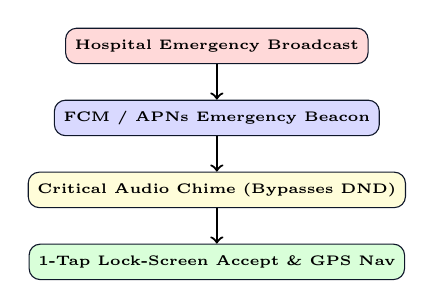
\begin{tikzpicture}[
                    node distance=0.45cm,
                    box/.style={rectangle, rounded corners, draw=DarkSlate, fill=white, font=\tiny\bfseries, minimum height=0.45cm}
                ]
                    \node[box, fill=red!15] (triage) {Hospital Emergency Broadcast};
                    \node[box, fill=blue!15, below=of triage] (fcm) {FCM / APNs Emergency Beacon};
                    \node[box, fill=yellow!15, below=of fcm] (chime) {Critical Audio Chime (Bypasses DND)};
                    \node[box, fill=green!15, below=of chime] (nav) {1-Tap Lock-Screen Accept \& GPS Nav};

                    \draw[->, thick] (triage) -- (fcm);
                    \draw[->, thick] (fcm) -- (chime);
                    \draw[->, thick] (chime) -- (nav);
                \end{tikzpicture}
                \end{center}
            \end{block}
        \end{column}
    \end{columns}
\end{frame}

% =============================================================================
\section{Verification \& Conclusion}
% =============================================================================

\begin{frame}{12. Implementation Verification \& Metrics}
    \begin{table}[H]
        \centering
        \small
        \begin{tabular}{llc}
            \toprule
            \textbf{Verification Layer} & \textbf{Test Suite / Command} & \textbf{Outcome} \\
            \midrule
            \textbf{Frontend TypeScript Build} & \texttt{tsc -b \&\& vite build} & \textbf{0 Errors (3.17s)} \\
            \textbf{REST API Endpoints} & Complete 18-Route Integration Matrix & \textbf{100\% Verified} \\
            \textbf{DBMS Integrity Checks} & Unique Compound Index \& Cascades & \textbf{Zero Orphan Records} \\
            \textbf{Design \& Responsiveness} & Minimalist Glassmorphism + Scroll-Lock & \textbf{Production-Ready} \\
            \bottomrule
        \end{tabular}
    \end{table}

    \begin{exampleblock}{\textbf{Summary of Technical Achievements}}
        \scriptsize LifeLink unites relational rigorousness (BCNF normalization, foreign key cascades, atomic inventory indexing) with modern micro-animated UX and geospatial donor discovery.
    \end{exampleblock}
\end{frame}

\begin{frame}
    \begin{center}
        \vspace{1.0cm}
        {\Huge \textbf{\textcolor{MedicalRed}{LifeLink Platform}}} \\[0.3cm]
        {\large \textbf{Bridging the Critical Gap in Emergency Blood Transfusion}} \\[0.8cm]
        \textbf{Thank You!} \\[0.4cm]
        {\small Questions \& Technical Discussion}
    \end{center}
\end{frame}

\end{document}
